\documentclass{vldb}
\usepackage{graphicx}
\usepackage{balance, url, amsfonts, verbatim, mathtools}  % for  \balance command ON LAST PAGE  (only there!)

\title{Probabilistically Bounded Staleness and\\ Practical Non-strict Quorum Systems}

\newdef{definition}{Definition}

\begin{document}

\interfootnotelinepenalty=10000
\hyphenation{prob-a-bil-is-tic-ally}

\maketitle

\noindent\textit{``All good ideas arrive by chance.''--Max Ernst}


\begin{abstract}

Modern storage systems employing quorum replication are often
configured to use partial, non-strict quorums.  These systems wait
only for a subset of their replicas to respond to a request before
returning an answer, without guaranteeing that read and write replica
sets intersect.  While these partial quorum mechanisms provide only
basic eventual consistency guarantees, with no limit to the recency of
data returned, these configurations are frequently ``good enough'' for
practitioners given their latency benefits. In this work, we discuss
why partial quorums are often acceptable in practice by analyzing the
staleness of data they return.  Extending prior work on strongly
consistent probabilistic quorums and using models of Dynamo-style
anti-entropy processes, we introduce Probabilistically Bounded
Staleness (PBS) consistency, which provides expectations of bounds on
staleness across both versions and wall clock time.  We derive a
closed-form solution for versioned staleness and model real-time
staleness for representative Dynamo-style systems under internet-scale
production workloads.  We quantitatively demonstrate why, in practice,
systems employing partial quorums often serve consistent data.

\end{abstract}


\section{Introduction}

Modern distributed storage systems need to be scalable, highly
available, and provide high performance for reads and writes.  These
systems typically replicate data across different machines or even
across datacenters for two reasons: first, to provide high
availability when components fail and second, to provide improved
performance by serving requests from multiple replicas.  In order to
provide predictably low read and write latency, systems often eschew
consistency across replicas and instead provide eventual
consistency. In this model, replicas are only guaranteed to eventually
agree on the value of a particular data item, and reads may return
arbitrarily stale data.

Distributed quorums are often used to ensure strong consistency across
multiple replicas of a data item by overlapping read and write
sets. However, service latency is critical. For example, at Amazon,
100 ms of additional latency resulted in 1\% drop in
sales~\cite{amazon-latency}, while 500 ms of additional latency at
Google due to increasing the number of search results computed
resulted in a corresponding 20\% decrease in search
traffic~\cite{google-talk}.  At scale, these decreases correspond to
billions of dollars of lost revenue.  To lower operation latency, data
system operators often employ \textit{non-strict or partial quorums},
in which read and write sets are not guaranteed to overlap (given $n$
replicas and read and write quorum sizes $r$ and $w$, $r+w \leq n$).
Modern quorum-based scalable data systems such as Dynamo~\cite{dynamo}
(and its open source descendants Cassandra~\cite{cassandra},
Riak~\cite{riak}, and Voldemort~\cite{voldemort}) provide two
categories of quorum operation: overlapping quorums and strong
consistency or variable-sized partial quorums with no guarantees on
the staleness or consistency returned, other than that the system will
``eventually'' provide the most recent version in the absence of new
writes. Further, operators of distributed storage system are required
to choose the a fixed size for the read and write sets which affects
the availability and latency of requests for a given workload.

\begin{comment}
\begin{figure}
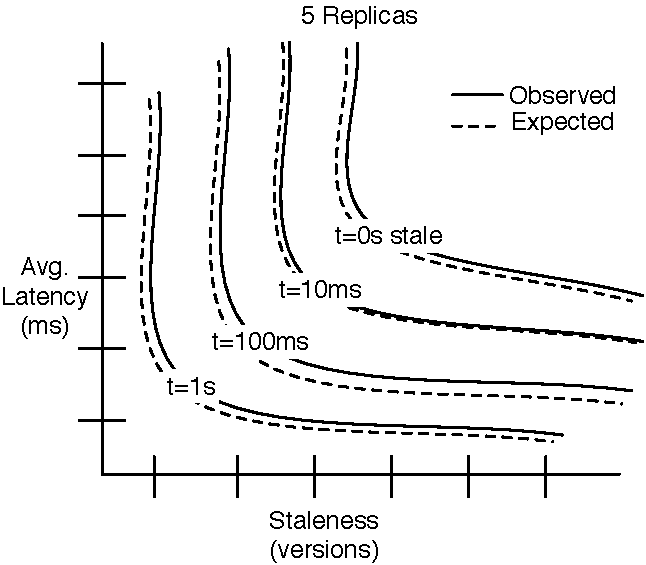
\includegraphics[width=.8\columnwidth]{figs/latency-stale.pdf}
\caption{In this work, we demonstrate the tradeoffs between latency
  and staleness (in versions and real-time) in quorum-based
  distributed databases.  This plot shows both modeled and empirical
  results along these axes for a quorum with $n=5$ replicas, $95\%$
  confidence, and equal rates of reads and writes. Moving along the
  curves corresponds to varying the read and write quorum
  sizes. Additional detail is given in Section~\ref{sec:eval}}
\label{fig:latency-staleness}
\end{figure}
\end{comment}

Prior theoretical work on \textit{probabilistic quorums} demonstrated
how partial quorums can be employed to provide arbitrarily high
probability of strong consistency~\cite{prob-quorum}. In theory, these
systems provide excellent asymptotic behavior but are limited in
practical applicability due to their reliance on high replication
factors.  Furthermore, in this theory, there is no guarantee on the
recency of data returned that is not strongly consistent (i.e., the
most recent version); with small $n$, the probability of this
happening is rather large---in the tens of percent.

In this paper, we present algorithms and models for accurately
predicting the staleness of a data item across multiple versions and
wall clock time, or Probabilistically Bounded Staleness (PBS). PBS
can be used to determine the probability of reading one of the last
$k$ versions of a data item, of reading a data item $t$ seconds after
it is written, and of experiencing a combination of the two.  We also
use these consistency measures to provide probabilistic guarantees on
monotonic reads, a form of session guarantees where reads are
guaranteed to return data items no older than what has been previously
read.  By analyzing the bounded-staleness consistency
constraints~\cite{vahdat-bounded} that arise naturally from the data store's
propagation algorithms, we provide quantitative insight into the
consistency-latency trade-offs they offer.

We demonstrate the trade-offs between consistency and performance and
show that these trade-offs need not be painstakingly experimentally
measured---they can be predicted.  Using a combination of simple
theory and online estimation, we can provide expected bounds on the
consistency of a data storage solution and optimize configuration
parameters accordingly.

\begin{comment}

By relaxing the consistency guarantees from strong consistency to a
bounded-staleness model(CITE) and by modeling write propagation
over time, or anti-entropic processes, we provide exponential
improvements in the probability of returning staler-than-promised
data.  This results in techniques that are useful at replication
levels as seen in practice ($n<10$, and easily $n\leq3$) and providing
quantitative insight into the consistency-latency trade-offs inherent
in these systems.

\end{comment}

Using this theory, we have developed a replica management policy that
determines the read and write quorum sizes ($w$,$r$,$n$) to optimize
the performance of an operation given the desired staleness bound. We
implement our policy in Cassandra, a widely-deployed open source
quorum-based distributed storage system and demonstrate how it can be
easily applied in practice. We validate our theory using several
microbenchmarks and worst-case sythetic workload and find that, for
latency distributions with means less than 15 milliseconds,
Dynamo-style systems provide strong consistency with extremely high
probability.

\begin{comment}
then demonstrate the
utility of staleness measures in a Twitter-clone with several thousand
clients.
\end{comment}

We make the following contributions in this paper:

\begin{itemize}

\item We develop the theory of Probabilistically Bounded
  Staleness (PBS) for partial quorums. PBS describes staleness
  probability metrics across both versions and time as well as
  probabilistic monotonic reads consistency
  (Section~\ref{sec:theory}).

\item We employ PBS theory under Dynamo-style~\cite{dynamo} quorum
  systems, the most widely deployed distributed quorum system
  mechanism, and describe how to calculate expected staleness.  We
  formulate a minimization of operation latency subject to a given
  service level agreement on the staleness of the data returned and
  the probability of further inconsistency
  (Section~\ref{sec:optimize}).

\item We implement this optimization layer and our algorithms as a
  policy system for a modern distributed key-value store and
  demonstrate its utility in practice under both synthetic
  benchmarking and worst-case stress tests (Section~\ref{sec:eval}).

\end{itemize}

\section{Motivation}

What kind of consistency do eventually consistent data stores provide?
At its core, eventual consistency is quite weak, only guaranteeing
that the latest write will not be lost and will, at some point in the
future, reside on all replicas.  Despite the weakness of this
guarantee, many systems opt only the most basic of eventual
consistency guarantees, with no bounds on the staleness of versions
observed.  To address this deficiency, a proliferation of proposed
systems fall across on of models in the consistency spectrum, from
session guarantees~\cite{session} to causal consistency to parallel
snapshot isolation~\cite{psi}.  However, many of the most widely
deployed systems do not provide these models; simple eventual
consistency is simple to implement, if difficult to reason about.
Rather than propose another consistency model external to existing
systems, we should provide better insight into how simple eventually
consistent systems operate.  We turn to the problem of diagnosing what
consistency our existing stores provide.

\textbf{Predictability.} Can we predict the staleness of
eventually-consistent data stores? However, eventually consistent data
stores often return fairly recent versions.  We should be able to
predict the staleness of values returned from our data stores.  This
ability would be invaluable for programmers, who might like to specify
constraints on the staleness of values in terms of versions,
wall-clock time, or both.  A streaming ``news feed''-style application
can tolerate some staleness, but staleness past an hour is likely
undesirable.

\textbf{Analysis.} How consistent are eventually consistent data
stores in practice?  There is a wide range of consistency models in
the academic literature, however many commercially-deployed data
stores have instead opted for weak eventual consistency or strong
consistency guarantees instead.  Ostensibly, these systems are working
well enough for their users; ``eventually'' does not mean infinite
time in practice.  It would be helpful to characterize when these data
stores are stale and understand under which conditions these data
stores are deficient.

\textbf{Configuration.} Using a prediction mechanism, can we
automatically configure our distributed data stores for a particular
workload?  Current database configuration...

\begin{comment}

There are two main reasons to replicate data across multiple servers:
availability and scalability.  First, in the event of network
partitions, replicas on separate sides of the partition can continue
to serve (possibly stale) data.  In the event of server failure
(effectively a single-node partition), having stored the data on
multiple replicas allows end-users to continue to access the data.
The replication factor in this case depends largely on the relative
``importance'', or cost of losing the data.  Second, and of central
importance to this work, each server has a maximum capacity, or number
of requests that it can serve within a given time period.  All else
equal, replicating the data and performing appropriate load-balancing
lowers the load on each individual server storing the data.  This has
the additional benefit of lowering read and write operation latency.

However, coordinating replicas has a cost; ensuring that all replicas
are up to date is expensive.  While the distributed databases
community developed designs and algorithms for ACID-style distributed
databases for decades (CITE), in light of massive scale, internet
services instead chose to move to so-called BASE semantics (CITE).  To
achieve availability and partition tolerance, BASE systems give up
consistency.  Indeed, BASE systems cannot have all of consistency,
availability, and partition tolerance at once~\cite{cap-proof}, yet
modern BASE systems (closely affiliated with the NoSQL ``movement''
(CITE)) drop many more guarantees regarding the data they return.
Many widely-deployed open source BASE systems drop transactional
support (CITE), complex schema (CITE), and even multi-key operations
(CITE).  These storage systems are often (initially, and certainly
conceptually) simpler than traditional distributed RDBMSs and, to
their credit, scale to hundreds or thousands of machines (CITE).

In the move to BASE semantics, many data management solutions have
thrown the baby out with the bathwater, providing the bare minimum of
guarantees on data consistency.  At its core, a guarantee of eventual
consistency is a guarantee that the latest write will not be lost and
will, at some point in the future, reside on all replicas.  There is a
wide and debatable set of points in the consistency spectrum
between the most basic of eventual consistency guarantees and strong
consistency, from session guarantees to parallel snapshot isolation to
causal+ consistency and others.  While there are indeed myriad
academic designs for less-than-strongly-consistent data stores, many
industrial eventually consistent data stores themselves have done a
poor job touting their own merits.  They promise either strong
consistency or basic eventual consistency, with no guarantees
in-between.

Despite providing only the most basic of guarantees, large, web-scale,
(often) highly profitable enterprises utilize eventually consistent
systems for production services every day (CITE, CITE, CITE).
Moreover, according to our interactions with system operators, many
services deploy their data systems with eventually consistent
guarantees.  Even with a lack of sophisticated guarantees, application
writers and systems operators use these systems: either they do not
understand or care about consistency or eventual consistency is good
enough in practice.  Rather than debase the architects and adopters of
eventually consistent data storage systems, we should instead better
understand \textit{why} and when eventually consistent is good enough
for them.

If we look deeper into the operation of eventually consistent data
stores, we can begin to answer this question.  While these data stores only
explicitly provide two modes of operation, in reality, they provide
gradations of consistency out of the box, without modification.  By
modeling their (simple) internal protocols, we can provide predictions
for the degree of consistency they provide.  We can use these
predictions to inform system deployment and warn programmers about the
likelihood of corner cases (or, depending on the configuration,
common-case inconsistencies).  We can understand when deployment
conditions dictate that ``eventually consistent'' means ``all bets are
off'' and when ``eventually consistent'' means ``almost always
strongly consistent''.  We shouldn't have to guess---and we don't need
to.

\end{comment}


\section{Probabilistically Bounded\\Staleness}
\label{sec:theory}

In this section, we introduce the theory of Probabilistically Bounded
Staleness to describe the consistency that existing eventually
consistent data stores provide.  PBS is an extension of prior work on
probabilistic quorums that accounts for staleness of both versions and
across time.  We introduce the notions of PBS $k$-quorums, which
stochastically bounds the staleness of versions returned by read
quorums, PBS $t$-visibility, which stochastically bounds the time
before a committed version appears to readers, and PBS $<k,
t>$-quorums, a combination of the two prior models.

\subsection{Quorum Foundations: Theory}

Quorum systems have long been proposed as a replication strategy for
distributed data storage.  Informally, a strict quorum system defines
a set of sets of nodes in a distributed system with the property that
any two sets in the quorum system overlap (have non-empty
intersection).  When considering distributed get/put operations,
reading and writing to sets of nodes in a strict quorum system ensures
strong consistency in the absence of failures; the minimum sized
quorum defines its fault tolerance.  A simple example of a strict
quorum system is the majority quorum system, in which each quorum is
of size $\frac{N}{2}+1$.  However, the theory literature contains
numerous alternative quorum systems providing varying asymptotic
properties of capacity, scalability, and fault-tolerance, from
tree-quorums to grid-quorums.  Jim\'{e}nex-Peris et. al provide a
useful overview of these traditional, strict quorum
systems~\cite{quorums-alternative}.

Non-strict quorum systems are a natural extension of strict quorum
systems: at least two sets in a non-strict quorum system do not
overlap.  There are two relevant variants of non-strict quorum systems in
the literature: probabilistic quorum systems and k-quorums.

\textit{Probabilistic quorum systems} provide probabilistic guarantees
on the consistency of data returned by non-strict quorums.
Probabilistic quorums provide optimal (expected) load and fault
tolerance with an arbitrarily small probability of
inconsistency~\cite{prob-quorum}.  Intuitively, this is a consequence
of the Birthday Paradox: as the number of replicas increases, the
probability of non-overlap between any two subsets is quite low.  To
the best of our knowledge, probabilistic quorums have only been used
to study the probability of strong consistency and have not been
employed in an eventually consistent context.

Given $n$ replicas and randomly chosen read and write quorums of sizes
$r$ and $w$, we can calculate the probability of the read quorum not
containing the value written by the write quorum.  The probability of
staleness is the number of quorums of size $r$ composed of nodes that
were not written to in the write quorum divided by the number of
possible quorums of size $r$:
\begin{equation}
\label{eq:prob-strict}
p_{stale}=\frac{{n-w \choose r}}{{n \choose r}}
\end{equation}
It is readily apparent that the probability of staleness is quite high
except for large values of $n$.  With $n=100$, $r=w=30$, $p_{stale} =
1.88 \times 10^{-6}$~\cite{nonstrict-availability}.  However, with
$n=3$, $r=w=1$, $p_{stale} = .\overline{6}$.  The asymptotics of these
systems are excellent---but only asymptotically.  

\textit{$k$-quorum systems} provide strong (non-probabilistic)
guarantees that the partial quorum system will return a value that was
written within $k$ versions of the most recent
write~\cite{nonstrict-availability}.  In the single-writer scenario,
one can imagine a round-robin write scheduling scheme where each write
is sent to $\frac{n}{K}$ replicas such that each replica is no more
than $K$ versions out-of-date.  However, with multiple writers, one
loses the ordering properties that the single-writer was able to
control, and the best known algorithm for the pathological case
results in a lower bound of $(2n-1)(k-1)+n$ versions staleness~\cite{k-quorum-lb}.
Again, this prior work on $k$-quorums focused on purely deterministic
verion staleness.

This prior work has two properties with important implications for
practitioners.  First, existing theory treats quorums as static; a
write quorum is chosen and no other replicas in the system
subsequently learn about the value unless it is written again.  The
theory does not account for propagation of versions across time and
between replicas (anti-entropic processes).  Second, much of this
prior work assumes Byzantine failure.  If the description of prior
work seemed simplistic, it is largely because most of the literature
content addresses problems such as adversarial quorum selection and
scheduling.  In this work, we disregard both of these assumptions.  We
elaborate further in the next section.

\subsection{Quorum Foundations: Practice}
\label{sec:practice}

In practice, many distributed data management systems employ variable
quorum sizes. Amazon's Dynamo~\cite{dynamo} is the progenitor of a
class of eventually-consistent key-value stores that provide
quorum-style replication that includes Apache Cassandra, Basho's Riak,
and LinkedIn's Voldemort\footnote{Other BASE-style systems may employ
  master-slave replication, as in Apache HBase~\cite{hbase}.}.  In
this paper, we discuss Dynamo-style quorum systems, particularly
because we are not aware of any significally different production
quorum data systems.  However, with some work, we believe that other
systems can adopt our methodology.  Similarly, we focus on key-value
stores as the aforementioned systems provide some variant of key-value
architecture and do not provide full RDBMS semantics.  Quorum systems
may be employed in RDBMS replication, but, for simplicity, we describe
key-value stores here.

Dynamo-style quorum systems employ one quorum system per key,
typically maintaining the mapping of values to a set of nodes using a
consistent-hashing scheme or a centralized membership protocol. Each
node acts as a replica for multiple keys.  Client read and write
requests are sent to a proxy node in the key-value store and are
subsequently forwarded by the receiving node to all other nodes
assigned to that key as replicas.  The proxy node acknowledges
operation success when it has heard from a pre-defined number of
replicas.  Dynamo-style systems return guaranteed strongly consistent
data when $R+W > N$.  However, for improved latency, operators often
set $R+W \leq N$, typically $R=W=1$, as is the default for these
database systems (see Table TBD).

\begin{figure}
\centering
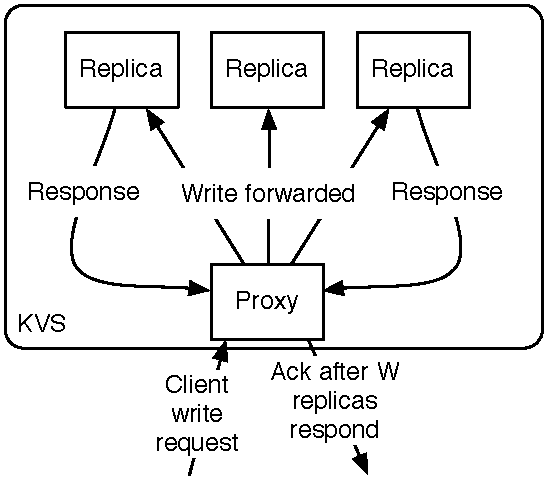
\includegraphics[width=.8\columnwidth]{figs/dynamo-quorum.pdf}
\caption{Diagram of control flow for client write to Dynamo-style
  quorum.  Here, $N=3$, $W=2$. Client writes are proxied and sent to
  all replicas. The write succeeds when $W$ replicas respond.  Note
  that the proxy is likely a replica as well, invoking a local write.}
\label{fig:dynamo-quorum}
\end{figure}

There are significant differences between data systems and the theory
describing quorum operation.  First, replication factors for
distributed data systems are relatively low.  Typical replication
factors are between one and three, however the literature has proposed
replication up to 10~\cite{chain-replication}.  Second, (in the
absence of failure), in Dynamo-style partial quorums, the number of
replicas that receive a write increases even after the operation
returns.  This is a simple version of anti-entropy.  Third, these
systems are often deployed in a trusted or semi-trusted computing
environment; there may be adversarial threats against data integrity
and denial-of-service attacks, but the underlying computing hardware
is non-adversarial. Within a controlled data center, the failure modes
are certainly reduced from the Byzantine case, and, despite its many
risks, the adversarial failures covered by prior theory appear
unlikely in emerging ``cloud computing'' environments.

\subsection{Assumptions}

These practical concerns guide the following theoretical
contributions.  Accordingly, we assume a quorum model where $w$ ($r$)
of $n$ replicas are randomly selected for each write (read) operation.
Unless otherwise noted, we consider fixed $w$ across multiple
operations.  We begin by considering a model without entropic
processes ($w$ is constant), then expand our model to consider
time-varying $w$. We consider a write ``committed'' once it has
reached $w$ replicas. We discuss further refinements to these
assumptions in Section \ref{sec:discussion}.

\subsection{PBS $k$-quorums}

Probabilistic quorums allow us to determine the probability of
returning the most recent value written to the database, but it is
also useful to know the probability of returning a value within a
bounded number of versions.  Deterministic $k$-quorums provide
theoretical approaches to achieving this, however we can do better in
the presence of multiple writers by extending this theory to consider
probabilistic $k$-quorums.  In this model, we consider static write
quorums (no anti-entropy), but compose multiple write quorums to model the probable overlap of $k$ independent write sets.
\begin{definition}
A quorum system obeys \textit{PBS $k$-quorum consistency} if, with
probability $1-p_{staler}$, at least one value in any read quorum will
have been committed no later than $k$ versions after the latest committed
version when the read begins.
\end{definition}
Versions whose writes that are not yet committed (in-flight) may be
returned by a read in this formulation of probabilistic $k$-quorums
(see Figure \ref{fig:timelines}A).  The $k$-quorum literature defines these as $k$-regular semantics~\cite{nonstrict-availability}.

\begin{figure}
\centering
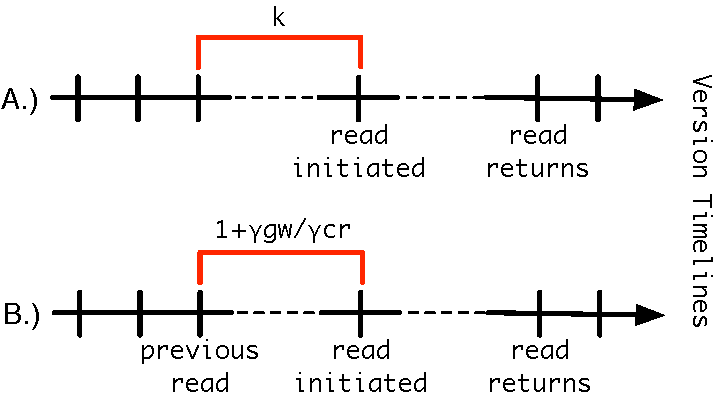
\includegraphics[width=\columnwidth]{figs/timelines.pdf}
\caption{Possible versions returned by read operations under
  PBS $k$-quorums (A) and PBS monotonic reads (B). In
  $k$-consistency, the read operation will return a version no later
  than $k$ versions older than the last committed value when it
  started; more versions may be committed during the read and may be
  returned.  In monotonic reads consistency, the staleness depends on
  the number of versions committed since the time the client last
  completed a read.  This is determined by the proportion of client's
  reads to the number of writes committed to the object.}
\label{fig:timelines}
\end{figure}

The probability of returning a version of a key within $k$ versions is
equivalent to intersecting one of $k$ independent write
quorums\footnote{In the language of probabilistic quorums, we have
  constructed a PBS $k$-quorum from $k$ $\varepsilon$-quorum
  systems where $\varepsilon \leq \sqrt[k]{p_{staler}}$. This system
  has load $\geq \frac{1-\varepsilon^{\frac{1}{2k}}}{\sqrt{n}}$, an
  exponentially lower bound than a strict probabilistic quorum.  This
  follows immediately from~\cite[Corollary 3.12]{prob-quorum}}.
Quorums are chosen at random, so the probability of non-intersection
is simply Equation \ref{eq:prob-strict} exponentiated by $k$:
\begin{equation}
\label{eq:k-consistency}
p_{staler} = \left(\frac{{n-w \choose r}}{{n \choose r}}\right)^k
\end{equation}

For the $n=3, r=w=1$ case, this means that the probability of
returning a version within $2$ versions is $.\overline{5}$, within $3$
versions $.\overline{703}$, and within $5$ versions $> .868$, and $10$
versions $>.98$.  With $n=3, r=1, w=2$ (alternatively, $r=2, w=1$),
these probabilities increase: $k=1 \rightarrow
.\overline{6}$, $k=2 \rightarrow .\overline{8}, k=5 \rightarrow >
.995$.

\subsection{PBS Monotonic Reads}

With additional information, we can use PBS $k$-quorums to
predict whether a client will ever read stale data.  This property,
known as \textit{monotonic reads} consistency is a well-known session
guarantee~\cite{sessionguarantees}.

\begin{definition}
\label{def:prob-mr}
A quorum system obeys \textit{PBS monotonic reads consistency} if, with probability at least $1-p_{staler}$, at
least one value in any read quorum the same version or a newer version
than the client's previously read value, where versions are defined
over the global commit ordering.
\end{definition}

To guarantee that a client sees monotonically increasing versions, it
can continue to contact the same replica~\cite{vogels-defs}, however
this is insufficient to guarantee strict monotonic reads (where the
client reads strictly newer data).  Definition~\ref{def:prob-mr} can
be adapted to acommodate strict monotonic reads (omitted for brevity).

We observe that monotonic reads is a special case of PBS
$k$-quorums where $k$ is determined by a client's rate of reads from a
data item ($\gamma_{cr}$) and the global, system-wide rate of writes
the same data item ($\gamma_{gw}$)\footnote{When constructed from $k$
  $\varepsilon$-consistent systems (as we have here), this consistency
  model has load $\geq
  \frac{(1-p_{staler}^{\frac{1}{2C}})}{\sqrt{n}}$, where
  $C=1+\frac{\gamma_{gw}}{\gamma_{cr}}$.}.  If we know these rates
exactly, the number of versions between client reads is
$\frac{\gamma_{gw}}{\gamma_{cr}}$, as shown in Figure
\ref{fig:timelines}B.  We can calculate the probability of
probabilistic monotonic reads as follows, effectively using Equation
\ref{eq:k-consistency} where $k=1+\frac{\gamma_{gw}}{\gamma_{cr}}$:

\begin{equation}
\label{eq:prob-mr}
p_{staler} = \left(\frac{{n-w \choose r}}{{n \choose r}}\right)^{1+\gamma_{gw}/\gamma_{cr}}
\end{equation}
For strict monotonic reads, exponentiate where $k=\frac{\gamma_{gw}}{\gamma_{cr}}$.

In practice, we may not know these exact rates, but, by measuring
their distribution, we can calculate an expected ratio that we can
integrate into these calculations.  However, by performing appropriate
admission control, operators can control these rates to achieve a
particular staleness target.

\subsection{PBS $t$-visibility}

Until now, we have considered only static write quorums.  However, as
we discussed in Section \ref{sec:practice}, modern quorum systems
propagate writes to all members of the quorum system for a given key.
This is commonly known as anti-entropy.  For generality, in this
section, we will discuss general anti-entropy models. However, we
explicitly model the Dynamo-style anti-entropy mechanism in Section
\ref{sec:dynamo-prop}.  PBS $t$-visible quorums model the
propagation of writes across wall-clock or real-world time such that
the set of replicas with a given version of the data (or later) grows
over time\footnote{Node failures shrink this set and can be
  incorporated into this model, but we do not consider them here.}.
We denote the cumulative density function describing the number of
replicas $\mathcal{W}$ that have a particular version $v$ (or a
version committed after $v$\footnote{We assume writes obey a total
  ordering. This can be accomplished using synchronized clocks (last
  writer wins) or with causal ordering and commutative merge
  functions~\cite{cops}.}) $t$ seconds after committing as
$P_w(\mathcal{W}, t)$.

\begin{definition}
A quorum system obeys \textit{PBS $t$-visibility consistency} if, with
probability $1-p_{staler}$, any read quorum started at least $t$ units
of time after the last version committed returns at least one value
that is at least as recent as the last version committed when the read
began (and may not be committed yet).
\end{definition}

By definition, $P_w(c,0) = 1$ $\forall c \in [0, w]$.  Intuitively, at
commit time, $w$ replicas will have the value, so the probability that
zero to $w$ replicas have the value immediately after commit is
exactly $1$.  We can model the probability of PBS $t$-visibility for an interval $t$ by summing the conditional probabilities of each possible $\mathcal{W}$:

\begin{equation}
p_{staler} = P_l(w, t)+\sum_{c\in(w, n]} \frac{{n-c \choose r}}{{n \choose r}}\cdot [P_w(c+1, t)-P_w(c,t)]
\end{equation}

In practice, $P_l$ depends on the expected latency of operations and can be
approximated analytically (Section \ref{sec:dynamo-prop} or measured
online\footnote{For this reason, it is difficult to analytically
  determine the load of any probabilistically consistent system
  dependent on real-time operations.}).

\subsection{PBS $\langle k, t
  \rangle$-quorum Consistency}

We can combine the previous models to combine both versioned and
real-time staleness metrics to answer questions of the following form:
what is the probability that a read will return a value no later than
$k$ versions old if the last write committed no sooner than $t$ seconds
ago?
\begin{definition}
A quorum system obeys \textit{probabilistic $\langle k, t
  \rangle$-quorum consistency} if, with probability $1-p_{staler}$, at
least one value in any read quorum will have been committed no later
than $k$ versions after the latest committed version when the read
begins, provided the read begins $t$ units of time after the previous
$k$ versions commit.
\end{definition}
The definition of $p_{staler}$ follows from the prior definitions:
\begin{equation}
p_{staler} = (P_l(w, t)+\sum_{c\in[w, n)} \frac{{n-c \choose r}}{{n \choose r}} \cdot [P_w(c+1, t)-P_w(c,t)])^k
\end{equation}
In this equation, we assume the pathological case where the last $k$
writes all occurred at the same time.  This is not likely in practice,
so if we can determine the time since commit for the last $k$ writes,
we can improve this staleness bound by considering each quorum's $p_{stale}$ at $RT=t$ separately.

Note that the prior definitions of consistency are encapsulated by
probabilistic $\langle k, t \rangle$-quorum consistency. probabilistic
$k$-quorum consistency is simply probabilistic $\langle k, 0
\rangle$-quorum consistency, probabilistic monotonic reads consistency
is $\langle 1+\frac{\gamma_{gw}}{\gamma_{cr}}, 0 \rangle$-quorum
consistency, and $t$-visibility is $\langle 0, RT \rangle$-quorum
consistency.

\section{Applying Theory to Practice}
\label{sec:optimize}

In this section, we discuss probabilitic quorums in the context of
Dynamo-style data storage systems.  We describe how to model the
probability of staleness in these systems as well as how to optimize
replica choice for a particular

\subsection{Dynamo-style Inconsistency}

Dynamo-style quorum systems are inconsistent as a result of read and
write message reordering.  Figure~\ref{fig:dynamostale} shows a
space-time diagram for messages between a sender and a single replica.
When reads and writes are executed, they are sent to all $N$

\begin{figure}
\centering
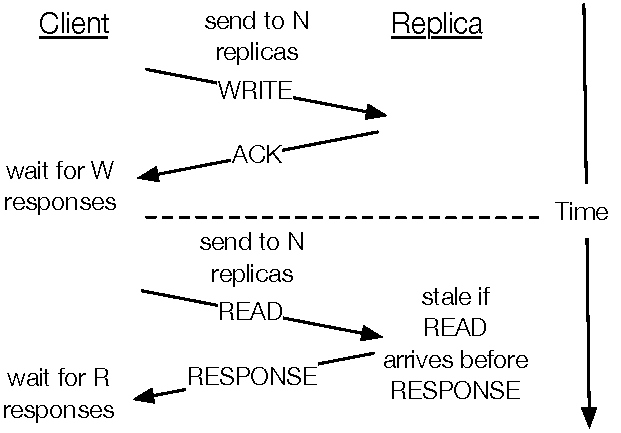
\includegraphics[width=.8\columnwidth]{figs/dynamostale.pdf}
\caption{Expected latency of write quorums of $w$ replicas in Dynamo-style operation versus quorum element correlation.}
\label{fig:dynamostale}
\end{figure}

\subsection{Dynamo-style Operation Latency}

\label{sec:dynamo-prop}

Until now, we have assumed that the expected latency of operations
reaching a given number of replicas by a particular time
($p_w(\mathcal{W}, t)$ for writes) in the case of writes is known.  We
can measure this distribution empirically (Section
\ref{sec:real-latency}), but we can also model this latency
analytically, given a few assumptions.

To begin, we consider write latency.  With Dynamo-style queries, we
want to determine the probability that $w$ of the replicas in the
write quorum $\mathcal{Q}$ respond within time $t$.  We can determine
this in at least two ways.  One way is to find use order statistic
theory to determine the probability that the $w$th replica reasponds
by time $t$.  However, this is equivalent to taking the minimum
response time over the maximum of each possible set of $w$ replicas
from $\mathcal{Q}$, which works out more cleanly in this formulation.
Given the write latency cumulative density functions for a set of
nodes $S$, $L_{ws}(S, t)$, the probability density function $p_w$ of
write latency of a set of nodes is:
\begin{equation}
p_w(\mathcal{W}, t) = min(\{L_{ws}(S, t) \mid S \subseteq \mathcal{Q}, |S| = \mathcal{W}\})
\end{equation}

To determine the expected latency of a write to a quorum of size
$\mathcal{W}$, enoted $WQ_l(\mathcal{W})$, we simply need to consider
the conditional probability of $\mathcal{W}$ writes completing across
all possible time values $t$.  However, this depends on the
distribution of $L_{ws}(S, t)$, which requires some
assumptions. Determining the ordinal probability of a set of randomly
distributed variables (in our case, the minimum of all $L_{ws}(S,
t)$), is possible but is also fairly complicated.  The difficult
arises in determining the distribution of a given $L_{ws}(S)$.  If we
assume that all nodes in $S$ obey independent latency distributions,
this is tractible.  If we assume that they are dependent and therefore
obey a joint distribution, then, as $w$ grows, solving for this
probability becomes much more difficult~\cite{needed}.  Approximation
algorithms can assist here~\cite{needed}, but we can also make
simplifying assumptions about the distribution of these latencies.

If we assume that latencies are independently, identically distributed
(IID), that is, if each node obeys the same latency distribution and
each nodes latency is independent of the other nodes's latency, this
equation is greatly simplified.  Under IID assumptions, the time for a
write to reach every node in the quorum obeys a single latency
CDF\footnote{Note that this distribution only captures the request
  forward, not the round-trip time before the acknowledgement.  The
  replica can serve the data before it responds to the proxy.},
$L_w(t)$ (PDF, resp. $l_w(t)$).  The probability that $w$ nodes all
respond within time $t$ is simply $(L_w(t))^\mathcal{W}$, and the
minimum over all such of these sets is the CDF $P_w$:
\begin{equation}
P_w(\mathcal{W}, t) = 1-(1-(L_w(t))^\mathcal{W})^{n \choose \mathcal{W}}
\end{equation}
This is indeed simplifying, but it makes the theory much simpler.  We
discuss the validity of this IID assumption when we measure latencies
experimentally in Section \ref{sec:real-latency}.

Under the IID assumption, we can easily determine the expected
Dynamo-style write quorum operation latency:
\begin{equation}
WQ_l(\mathcal{W}) = \int_0^{\infty} t \cdot p_w(\mathcal{W}, t) dt
\end{equation}
In practice, the proxy is often a replica as well, so for a write
quorum of size $w$, we only need to consider $\mathcal{W}=w-1$ writes.

Similarly, to determine how many replicas have a particular value (even if they have not acked) after a write quorum of size $w$, we evaluate:
\begin{equation}
P_{w:have}(\mathcal{W}, t) = 1-(1-(L_w(t))^{\mathcal{W}-w})^{n-w \choose \mathcal{W}-w}
\end{equation}

Thus far, we have only considered the write operation latencies.  The
read quorum latency may be different from the write latency depending
on node-level actions such as forced logging or disk-bound operations.
However, the expected read operation latency for a quorum of size
$\mathcal{R}$, $RQ_l(\mathcal{R})$, can be calculated similarly given a
model for the latency of reads ($L_{rs}(S,t)$ and $L_r(t))$.

\subsection{Optimization Formulation}

With these equations, we can optimize the selection of a partial
quorum system to minimize overall operation latency subject to
constraints on staleness. We can guarantee bounded staleness by
ensuring that $p_{staler} = 1$, however this is only possible in
$k$-quorum consistency as the real-time components of $RT$-quorum
consistency and its variants are inherently probabilistic (unless we
can prove an absolute bound on operation latency).  We can use a
simply formulated optimization program to determine what combination
of $r$ and $w$ minimizes latency while satisfying the system
constraints and user requirements.

Given $n$, desired $p$, $w_{min}$ (minimum durability of writes),
consistency model (with necessary parameters--$k$, $t$, $\gamma_{cr}$,
etc.), and the relative weighted ``importances'' of read
and write latency, $c_r$ and $c_w$, we can determine $r$ and $w$:

\begin{equation}
 \begin{array}{rl}
    \min        & c_r\cdot RQ_l(r) +c_w \cdot WQ_l(w) \\
    \mbox{s.t.} & p \ge p_{staler} \\
                & w \ge w_{min}.
    \end{array}
\end{equation}

We implement and validate this optimization framework in
Section~\ref{sec:optimization}.

\subsection{Typical Quorum Configurations}

CASSANDA: R=1, W=1 

<<<<<<< HEAD
RIAK: N=3, R,W QUORUM 
=======
RIAK: N=3, R,W QUORUM \url{https://github.com/basho/riak_kv/blob/1.0/src/riak_kv_app.erl}
\url{http://wiki.basho.com/Riak-Glossary.html#Quorum}
>>>>>>> 11fb27c39c7f11f1b544d903fd16543cac89854b

Voldemort: does not provide production configs besides testing (N=2)

\section{Experimental Evaluation}
\label{sec:eval}

We evaluated Dynamo-style partial quorums through the lens of PBS.  We
first implemented PBS policies on top of an open source Dynamo clone,
Cassandra, and compared our theory to observed results in a cloud
computing environment.  We subsequently predicted and measured and
predicted the PBS $k$-quorum and $t$-visibility consisistency across
several environmental configurations.

\subsection{Implementation}

We implemented PBS policies on top of Cassandra, an open source data
management system.  Cassandra provides Dynamo-style partial quorum
semantics, offering per-request quorum sizes and a BigTable-like
schemas~\cite{needed}.  Our changes to Cassandra were minimal: we
added support for partial quorums of size greater than
three---requiring changes to the wire protocol and request handling
code---and instrumented parts of the database to provide timing
information about reads and writes.  By analyzing Cassandra logs, we
were able to reconstruct the latency distributions of write requests,
write acknowledgements, read requests, and read responses.

READ REPAIR: DEPENDENT ON READ AND WRITE

We disabled read repair in Cassandra.  When a read quorum returns
divergent versions, we return the highest-valued version and do not
attempt read repair, essentially writing the new value back to the
stale replicas.  For a read request, Cassandra sends out a read
request to one node and ``digest'' requests for hashes of data items
to $R-1$ replicas on a read request.  If there is a mismatch between
any digest and the value read, Cassandra begins read repair, incurring
another set of round trips between the read coordinator and the
replicas.  We disable this feature and send out vanilla read requests
to all replicas instead.  Accordingly, we overestimate the staleness
of versions returned.

We implemented a staleness predictor using Monte Carlo simulation.
The closed-form solution is tractable, but there are several reasons
why we preferred simulation.  Simulating the message delays is simple.
One simply has to draw from each distribution and compare latencies to
determine the degree of staleness.  The Dynamo model is easily
implemented in an event-based simulation.  The analytical model is
much more complicated.  We found that implementing the analytical
model is rather onerous, requiring a large amount of numerical
integration and difficult code.  This is potentially a barrier for
adoption for practitioners.  Finally, when operating over discrete,
experimentally-gathered distributions (without curve-fitting), Monte
Carlo simulation was significantly faster.  Accordingly, our predicted
results here are derived from repeated simulation trials.

\subsection{Experimental Deployment}

We deployed Cassandra on Amazon EC2.  To provide a single point of
order for the series of reads and writes in the system, we deployed
$N+1$ Cassandra nodes for each experiment involving $N$ nodes.  After
configuring the Cassandra schema, we determined the node that did not
store the data and sent all requests through it, effectively creating
a remote proxy.  Our model is more general than the specific proxy
configuration, however using a centralized proxy allows us to avoid
most issues with clock skew between replicas and rely less heavily on
globally synchronized clocks.

We used \texttt{m1.small} instances throughout our experiments within
the \texttt{us-east-1} availability zone.  To model network and remote
processing delays, we injected delays into both the request and
response sending modules in Cassandra.  We discuss our choice of
distributions and their effects in Subsection~\ref{subsec:delay}.

\begin{comment}

One major challenge in performing our experiments was the possibility
of clock skew across replicas; we relied on synchronization between
the Xen hypervisors running our virtual machines.

\end{comment}

\subsection{Observed Staleness}

We issued reads and writes to a single key distributed across a
Cassandra cluster and measured the observed staleness.  While we ran
multiple configurations, to begin, we will discuss the configuration
where $N=3$, $R=1$, and $W=1$, Cassandra's default settings.

With a single reader and a single writer, under normal operation, we
observed little to no staleness.  Reads completed in 2.59 ms (99th
percentile: 30.61 ms) and writes completed in 2.34 ms (99th
percentile: 22.36 ms).  This was too narrow a window to observe the
message reordering required for any staleness.  However, our experiment is somewhat synthetic

\begin{figure}
\centering
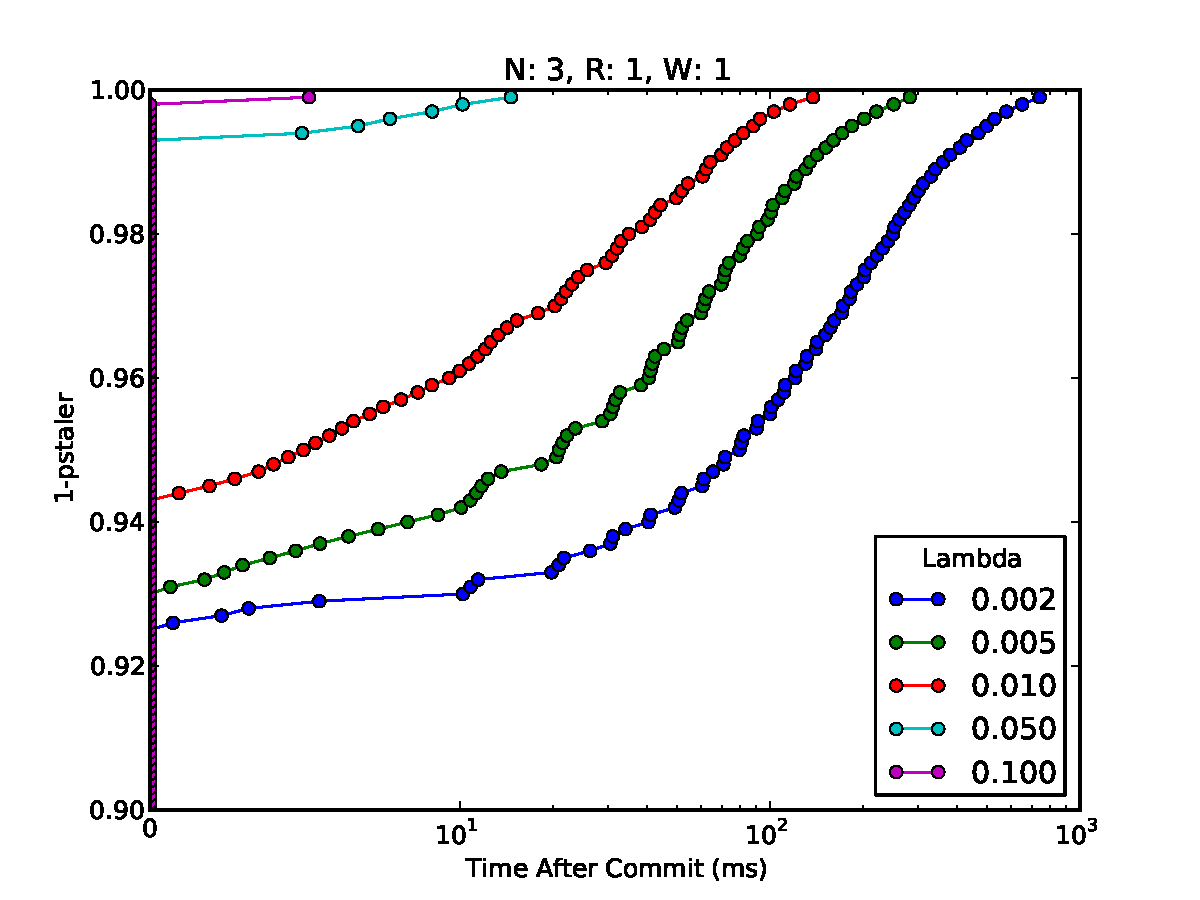
\includegraphics[width=.8\columnwidth]{figs/t-cdf.pdf}
\caption{Expected latency of write quorums of $w$ replicas in Dynamo-style operation versus quorum element correlation.}
\label{fig:correlation}
\end{figure}


\begin{figure}
\centering
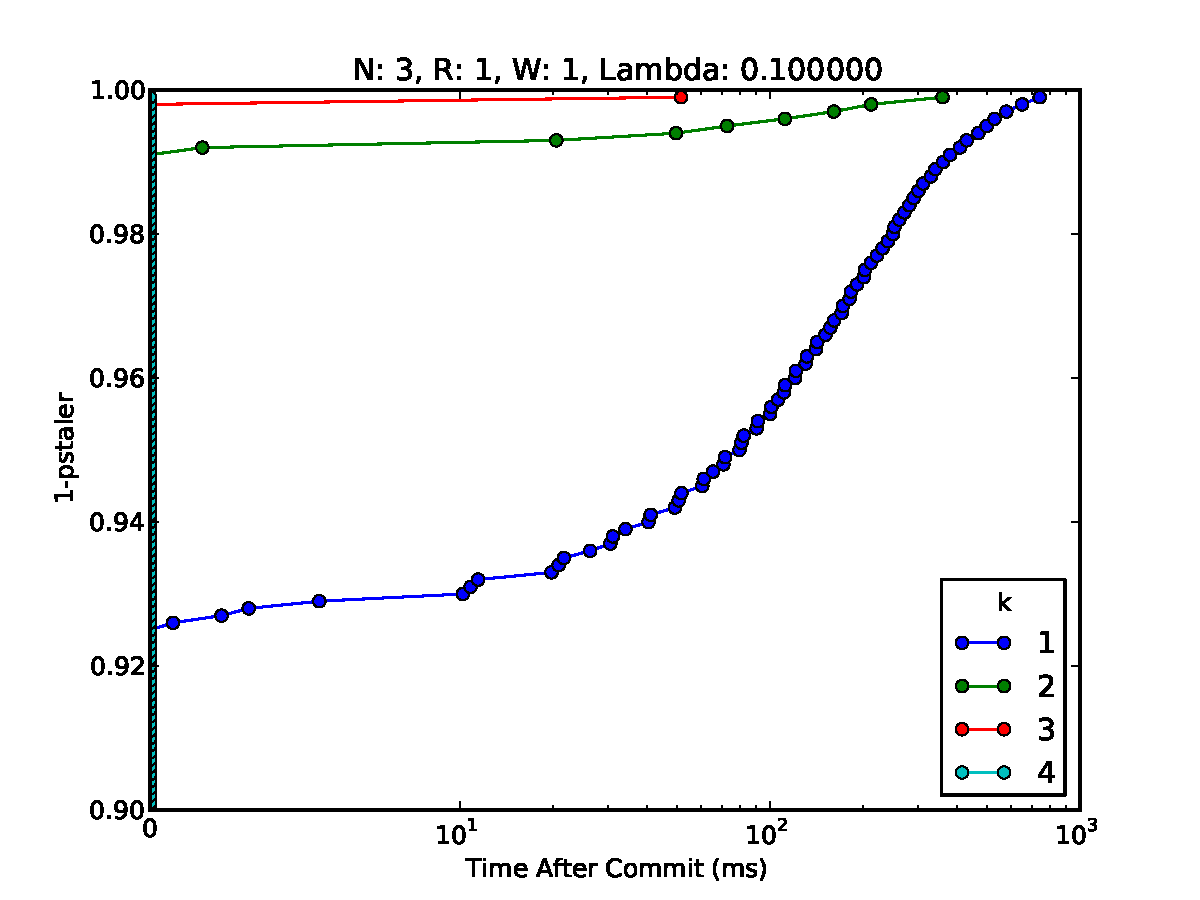
\includegraphics[width=.8\columnwidth]{figs/t-cdf-k.pdf}
\caption{Expected latency of write quorums of $w$ replicas in Dynamo-style operation versus quorum element correlation.}
\label{fig:correlation}
\end{figure}


\begin{figure}
\centering
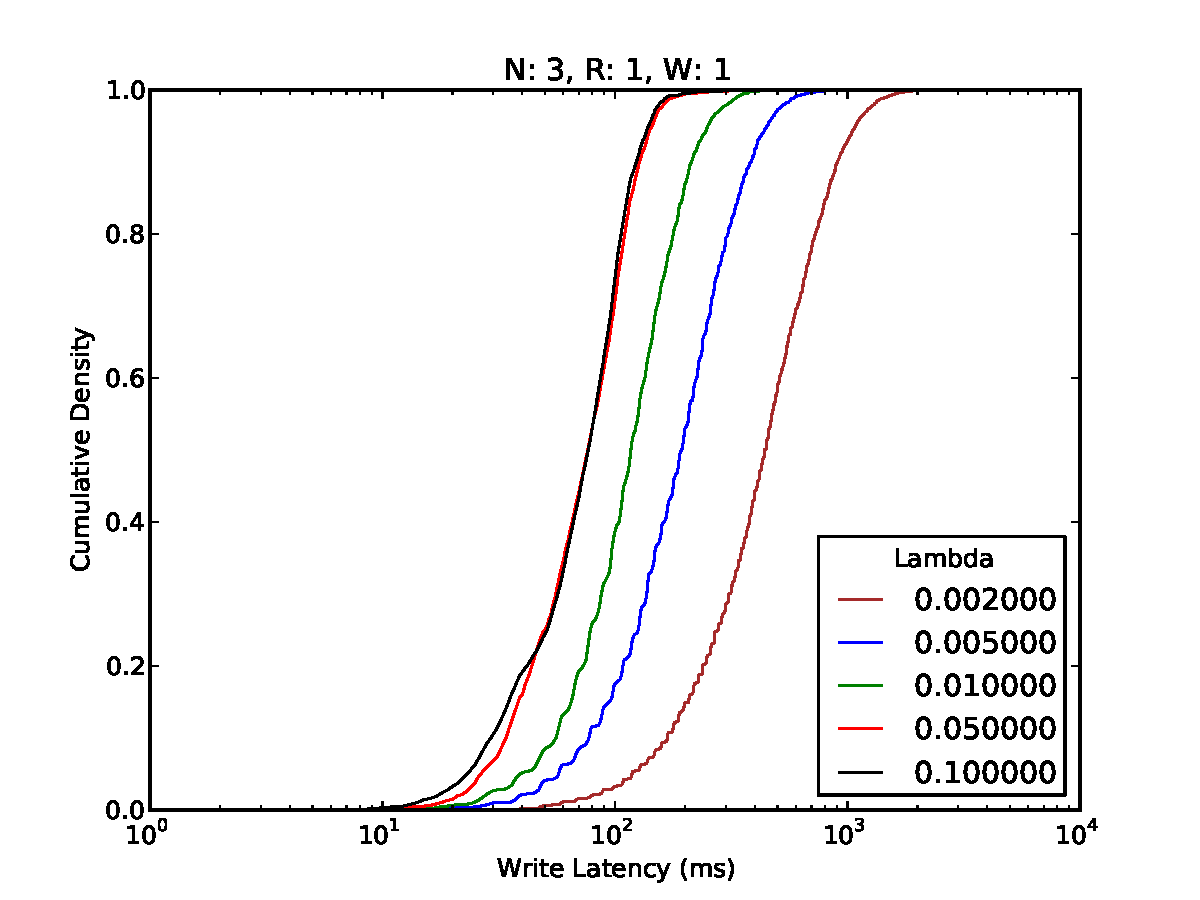
\includegraphics[width=.8\columnwidth]{figs/write-cdf.pdf}
\caption{Expected latency of write quorums of $w$ replicas in Dynamo-style operation versus quorum element correlation.}
\label{fig:correlation}
\end{figure}




\begin{comment}

N: 3 R: 1 W: 2 lambda 0.000000
Avg write latency: 2.340356 (stddev: 3.320391, 99th %ile: 22.360338)
Avg read latency: 2.588911 (stddev: 6.489868, 99th %ile: 30.617551)

N: 3 R: 1 W: 3 lambda 0.000000
Avg write latency: 4.412850 (stddev: 8.626731, 99th %ile: 50.466737)
Avg read latency: 2.277779 (stddev: 6.003202, 99th %ile: 28.037702)

N: 3 R: 2 W: 1 lambda 0.000000
Avg write latency: 1.786696 (stddev: 2.229738, 99th %ile: 6.011726)
Avg read latency: 2.047036 (stddev: 5.385266, 99th %ile: 23.046278)

N: 3 R: 2 W: 2 lambda 0.000000
Avg write latency: 2.314494 (stddev: 3.058672, 99th %ile: 16.398516)
Avg read latency: 2.068930 (stddev: 5.495067, 99th %ile: 22.539867)

N: 3 R: 3 W: 1 lambda 0.000000
Avg write latency: 1.869139 (stddev: 3.258769, 99th %ile: 14.491754)
Avg read latency: 3.309529 (stddev: 8.348639, 99th %ile: 44.156379)

\subsection{Operation Latency}
\label{sec:real-latency}

In our measurements on EC2, the correllation of writes was MADE UP,
meaning the operations were effectively IID.  However, we can
approximate an environment with a higher correlation by modifying $w$.
In an environment where half of the nodes are co-located on a rack, we can treat $w$ as $w/2$.  We show the tradeoffs between correlation and latency in Figure \ref{fig:correlation}.

\begin{figure}
\centering
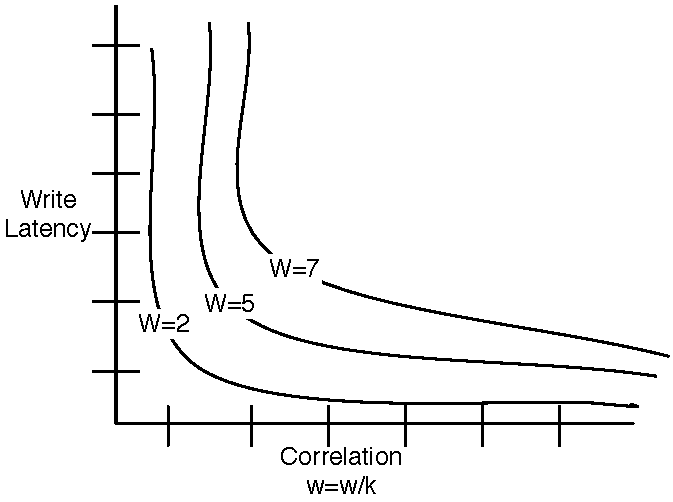
\includegraphics[width=.8\columnwidth]{figs/correlation.pdf}
\caption{Expected latency of write quorums of $w$ replicas in Dynamo-style operation versus quorum element correlation.}
\label{fig:correlation}
\end{figure}

\subsection{Optimization and SLAs}
\label{sec:optimization}

\begin{figure}
\centering
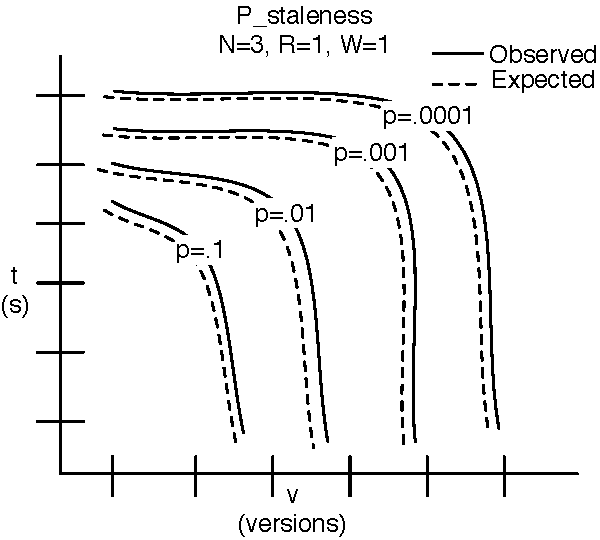
\includegraphics[width=.8\columnwidth]{figs/bothdimensions.pdf}
\caption{Time and version staleness required to ensure varying SLA constraints on the probability of returning staler-than-promised data in simple microbenchmarking.}
\label{fig:prob-staler}
\end{figure}

\begin{figure}
\centering
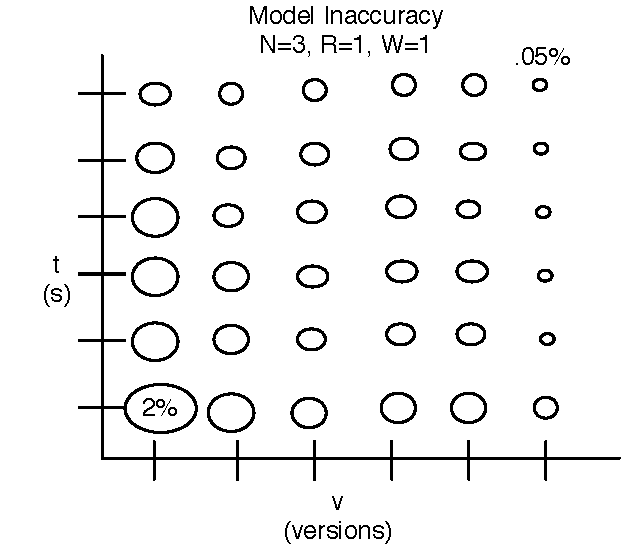
\includegraphics[width=.8\columnwidth]{figs/inaccuracy.pdf}
\caption{Accuracy of model compared to experimental microbenchmarking.
  The size of each point is linearly proportional to the inaccuracy of
  the model's predictions.}
\label{fig:prob-staler}
\end{figure}




\subsection{Twitter Clone}

\begin{figure}
\centering
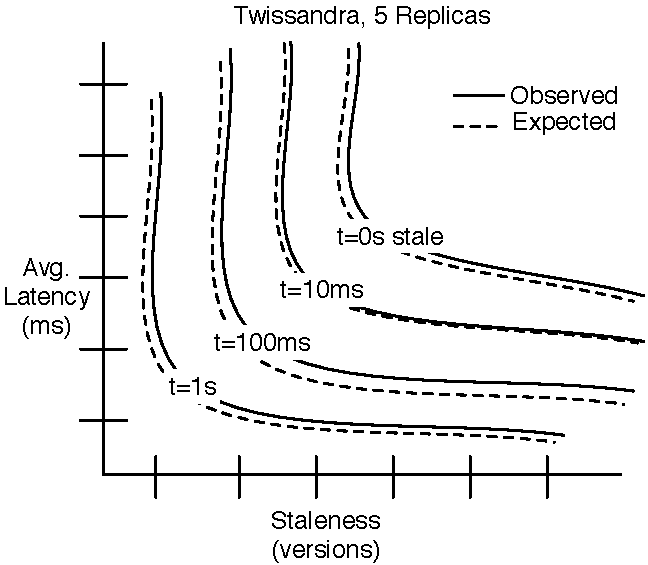
\includegraphics[width=.8\columnwidth]{figs/twissandra.pdf}
\caption{Time and version staleness tradeoffs as measured by end users
  of Twitter clone.}
\label{fig:twissandra}
\end{figure}

\end{comment}

\section{Discussion}
\label{sec:discussion}

There are several aspects of distributed data systems that we have not yet
addressed.  Here, we briefly discuss improvements to our models.

\subsection{Is Eventually Consistent Good Enough?}

One Cassandra committer noted that although he had a patch for session guarantees, no Cassandra users had requested the functionality or claimed to require it.

\subsection{Additional Functionality}

READ-MODIFY-WRITE

\textbf{Staleness detection.} Each of the $p_{staler}$ bounds
describes a probability that a particular key is no staler than
specified.  In the context of probabilistic consistency SLAs, it would
be useful to determine whether a key is staler than promised by a
given SLA.  Determining this fact on-line is tantamount to achieving
strong consistency, however there are at least two strategies for
mitigating this difficulty. First, additional gossiping such as
regular negative acknowledgements can notify nodes of potential
version staleness.  This strategy has been discussed in the
literature~\cite{tocite} for non-probabilistic quorum systems.
Second, the system can provide asychronous notifications of staleness
information.  Proxies can keep a growing log of versions which, with
appropriate timestamping, can be used to determine if previously
returned values were staler than promised.  This is fairly
straightforward but requires careful garbage collection to manage
proxy-side state as the number of client requests scales.
Additionally, the possibility of proxy failure requires that prior
operations be durably logged; however, provided the proxy eventually
comes online and updates its log, the asynchronous guarantee holds.
Both of these schemes are feasible yet add significant complexity to a
probabilistically consistent quorum system.

\textbf{Multi-key transactions.} We have considered single-key operations,
however the ability to perform distributed transactions is potentially
attractive.  For read-only transactions, if the key distribution is
random, each quorum is independent, so we can simply multiple the
staleness probabilities of each key.  Achieving atomicity of writes to
multiple keys requires more complicated coordination mechanisms such
as two-phase commit.  Again, transactions are feasible but require
considerable care in implementation, complicated what is otherwise a
simple replication scheme.

\textbf{Node failures.} Fail-stop node failures can be easily
incorporated into our latency models. The probability of a node
permanently failing $p_{f-perm}$ can be represented by setting the
probability of infinitely long read and write
operations. $L_{w}(\inf)=L_{r}(\inf)=p_{f-perm}$.  Intermittent node
failures of length $t_{fail}$ can be represented by setting
$L_{w}(t_{fail})$ to the probability of the node failing.  In this
way, operation latency captures all expected failure semantics.

\textbf{Read repair and active anti-entropy.} Modern Dynamo-style
systems use a technique known as \textit{read repair} to reconcile
divergent versions at query-time.  If two nodes return different
responses to a \textit{get} request, the responses are merged and
forwarded to the determined out-of-date node.  Dynamo performs
additional anti-entropy using Merkel trees, however the open source
databases we have examined only perform read repair (CITATION
needed--at least Cassandra does this). We do not model read repair or
additional anti-entropy processes here (although doing so requires
only minimal changes to our model), so we overestimate the chance of
staleness violation.

\textbf{Variable $w$.} We have assumed the use of a single $w$ across
all writes.  However, many KVSs such as Cassandra and Riak allow the
use of per-operation consistency\footnote{Voldemort specifies
  consistency requirements at the schema level. This is ostensibly an
  engineering decision that could be changed with minimal
  modifications to the wire protocol.}

\textbf{99th Percentile Latency.}


\section{Related Work}

Theory

Vadhat

\section{Conclusion}

\section*{Acknowledgements}

\balance

\bibliographystyle{abbrv}
\bibliography{ernst}

\begin{appendix}
\section{Dynamo-style Staleness}

We present an analytical closed-form solution to $p_{staler}$ for
$t$-visible partial quorums unde Dynamo-style.  What is the
probability that a read result is not strongly consistent (that is,
does not return the most recent value when the read began)? In this
section, when we refer to the ``last committed version'', we are
referring to the last committed version before the read began. We
consider the pathological case where a read occurs immediately after a
write occurs.

We assume that each writes to a replica is independently delayed by a
randomly distributed variate $W$, each write acknowledgement from a
replica to a writer is independently delayed by a randomly distributed
variate $A$, each read request to a replica is independently delayed
by a randomly distributed variate $R$, and each read response from a
replica to a reader is delayed according to a randomly distributed
variate $S$.  We make no assumptions as to the distribution of $W,$
$A,$ $R,$ and $S$, except that their domain is strictly positive (no
negative delay) and that values drawn from each are independently,
identically distributed (IID).

The probability that a read quorum does not contain the last committed
version is equivalent to the probability that each of the first $R$
read responses are all stale.  Denote the probability that the $i$th
response is stale as $stale_i$:
\begin{equation*}
p_{staler} = \prod_{i=0}^{R} \Pr(stale_i)
\end{equation*}

Denote the return time of the $i$th read response as $S_i$.  The probability that the $i$th response is stale is given by:
\begin{equation*}
\Pr(stale_i) = \int_{0}^{\infty} \Pr(S_i = t) \cdot \Pr(stale_i \mid S_i = t) dt
\end{equation*}

We can use simple order statistics to calculate the return time of the $i$th read response:
\begin{multline*}
\Pr(S_i = t) = \frac{N!}{(i-1)!(N-i)!}\cdot[\Pr(R+S< t)]^{i-1}\\\cdot\Pr(R+S = t)\cdot[\Pr(R+S > t)]^{N-i}
\end{multline*}

 Recall that under Dynamo-style messaging, read response from a
 replica is stale if the read request arrived at the replica before
 the write command for the last committed version reached the replica.
 Denote the time required to commit the last version (alternatively, the time required for $W$ of $N$ replicas to acknowledge the last write) as $w_t$.
\begin{multline*}
\Pr(stale_i \mid S_i = t) = \int_{0}^{t} \Pr(R=\tau)\cdot\Pr(S=t-\tau)\\\cdot\Pr(R+w_t < W \mid R = \tau) d\tau
\end{multline*}
\begin{multline*}
  \Pr(R+w_t < W \mid R = \tau) = \int_{\tau}^{\infty} \Pr(W-w_t = x) dx
\end{multline*}
\begin{multline*}
  \Pr(W-w_t = z) = \int_{0}^{\infty} \Pr(W = y) \cdot \Pr(-w_t = z-y) dy
\end{multline*}
Finally, to calculate $w_t$, we calculate the probabilty that
$\mathcal{W}$ of $N$ acknowledgements come in at time $t$:
\begin{multline*}
\Pr(w_t = t) = \frac{N!}{(\mathcal{W}-1)!(N-\mathcal{W})!}\cdot[\Pr(W+A< t)]^{\mathcal{W}-1}\\\cdot\Pr(W+A = t)\cdot[\Pr(W+A > t)]^{N-\mathcal{W}}
\end{multline*}
Combining these equations, we have a closed-form solution for the
staleness dependent on $W,$ $A,$ $R,$ and $S$, as desired.  To consider
multiple version staleness, exponentiate $p_s$ by the number of
versions stale.

\end{appendix}

\end{document}

